% !Mode:: "TeX:UTF-8" 

\BiChapter{模板的其它说明}{Other explanation about the template}

\BiSection{英文封面}{English cover}

英文封面下方的学位论文相关信息可以采用~\verb|tabular|~和~\verb|tabularx|~两种表格环境,具体使用哪一种环境和具体的相关信息有关。若信息内容不太长,不会引起信息内容分行时,则应该采用~\verb|tabular|~环境;若信息内容过长,会引起信息内容分行时,则应该采用~\verb|tabularx|~环境。具体用法请见~format.tex~文件的相应代码。

\BiSection{单层罗列环境}{Monolayer list environment}
哈工大学位论文一般可采用两种罗列环境:一种是并列条目有同样标签的~\verb|itemize|~罗列环境,另一种是具有自动排序编号符号的~\verb|enumerate|~罗列环境。这两种罗列环境的样式参数可参考图~\ref{list}。
\begin{figure}[htbp]
\centering
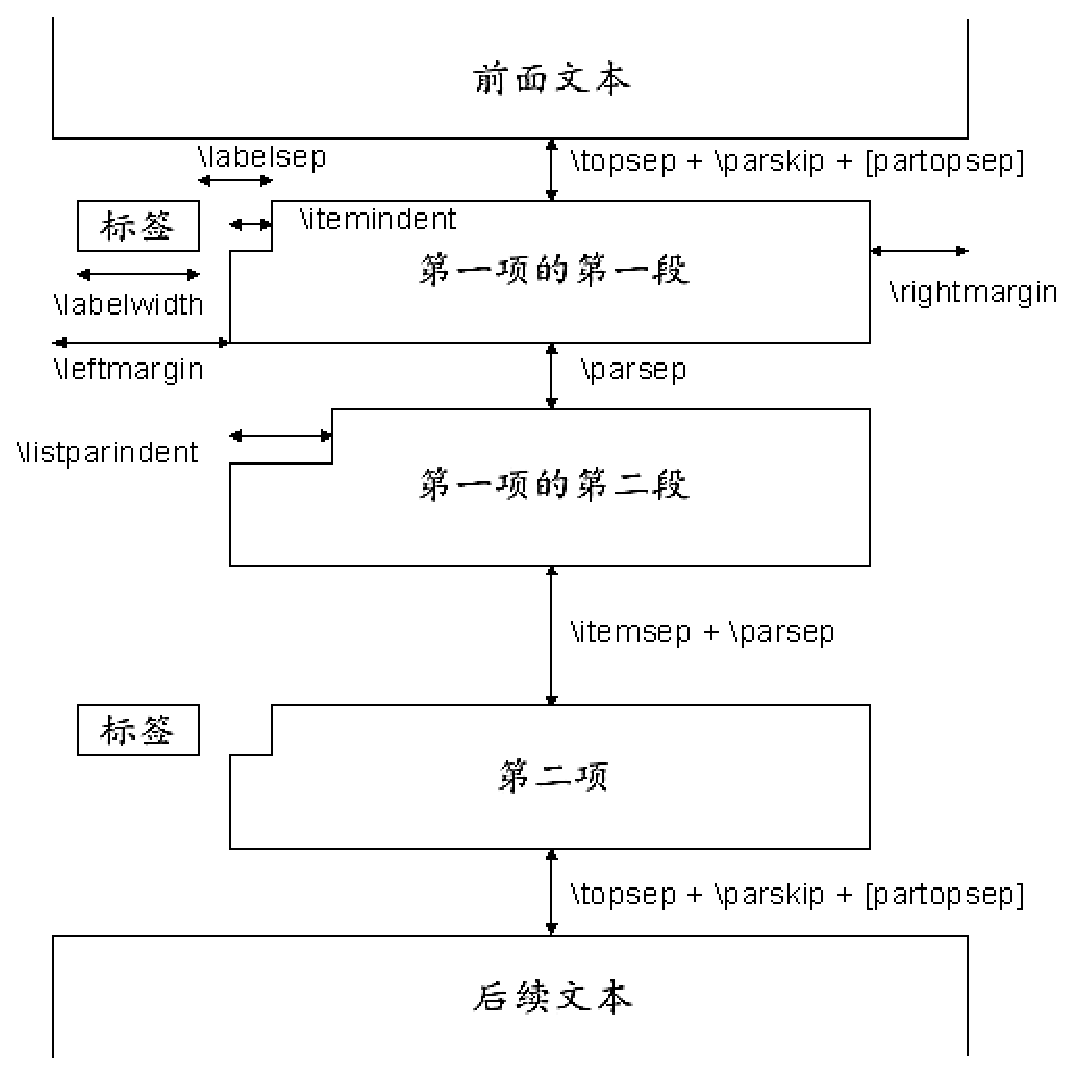
\includegraphics[width = 0.6\textwidth]{list}
\bicaption[list]{}{罗列环境参数示意图}{Fig.$\!$}{Schematic diagram of list environments}\vspace{-1em}
\end{figure}
通过调用~enumitem~宏包可以很方便地控制罗列环境的布局,其~format.tex~文件中的~\verb|\setitemize|~和~\verb|\setenumerate|~命令分别用来设置~\verb|itemize|~和~\verb|enumerate|~环境的样式参数。采用~\verb|itemize|~单层罗列环境的排版形式如下:
\begin{itemize}
\item 第一个条目文本内容
\item 第二个条目文本内容
\item 第三个条目文本内容
\end{itemize}
其代码如下
\begin{verbatim}
\begin{itemize}
  \item 第一个条目文本内容
  \item 第二个条目文本内容
  ...
  \item 第三个条目文本内容
\end{itemize}
\end{verbatim}
采用~\verb|enumerate|~单层罗列环境的排版形式如下:
\begin{enumerate}
\item 第一个条目文本内容
\item 第二个条目文本内容
\item 第三个条目文本内容
\end{enumerate}
其代码如下
\begin{verbatim}
\begin{enumerate}
  \item 第一个条目文本内容
  \item 第二个条目文本内容
  ...
  \item 第三个条目文本内容
\end{enumerate}
\end{verbatim}

\BiSection{算法}{Algorithm}

这是一个算法的例子,来自~worldguy@lilacbbs。建议将算法放在~minipage~环境中,避免算法出现在页面版心之外。

\begin{algorithm}
\KwIn{training samples, {$(d_i, d_j)_q$; $\mathbf{q}_i, \mathbf{q}_j \in C$,
$q\in \mathbf{Q}$} }
\KwOut{parameter setting $\lambda^T$}%

\For{$t$=1 to $T$}
{   
    $\lambda^{t+1}_n = \lambda^t_n + \eta (f_n(q, c, d_i) - f_n(q, c, d_j))$
 }
\end{algorithm}

%\KwIn{training samples, {$(d_i, d_j)_q$; $\mathbf{q}_i, \mathbf{q}_j \in C$,
%$q\in \mathbf{Q}$} }
%\KwOut{parameter setting $\lambda^T$}%
%
%\For{$t$=1 to $T$}
%{   
%    $\lambda^{t+1}_n = \lambda^t_n + \eta (f_n(q, c, d_i) - f_n(q, c, d_j))$
% }
%\end{algorithm}

算法环境中右侧空白比较多,若想把右侧的空白框减小,可以采用~minipage~环境实现。把~algorithm~环境放到~minipage~环境里面,并且加上选项[H]禁止算法浮动,下面给出一个例子。需要说明的是,一般不需要进行这种处理。算法标题可有可无,若有中英文标题,请使用~\verb|\AlgoBiCaption{中文标题}{英文标题}|。下面给出两个有标题的例子。需要说明的是,算法的标题是自动换行,没有必要手动换行。

\begin{minipage}{0.8\textwidth}\centering
\begin{algorithm}[H]
 \AlgoBiCaption{这是一个简短的算法中文图题}{This is the English caption of the algorithm}
  \KwIn{training samples, {$(d_i, d_j)_q$; $\mathbf{q}_i, \mathbf{q}_j
      \in C$, $q\in \mathbf{Q}$} }
 \KwOut{parameter setting
    $\lambda^T$}
 \For{$t$=1 to $T$} { $\lambda^{t+1}_n = \lambda^t_n +
    \eta (f_n(q, c, d_i) - f_n(q, c, d_j))$ }
\end{algorithm}
\end{minipage}


\begin{minipage}{0.9\textwidth}\centering
\begin{algorithm}[H]
 \AlgoBiCaption{这是一个算法的比较长的中文图题,需要换行,这里采用自动换行,如果手动换行会造成算法目录中同样出现断行}{This is a long English caption of the algorithm, a new line  required, and this a new line}
  \KwIn{training samples, {$(d_i, d_j)_q$; $\mathbf{q}_i, \mathbf{q}_j
      \in C$, $q\in \mathbf{Q}$} }
 \KwOut{parameter setting
    $\lambda^T$}
 \For{$t$=1 to $T$} { $\lambda^{t+1}_n = \lambda^t_n +
    \eta (f_n(q, c, d_i) - f_n(q, c, d_j))$ }
\end{algorithm}
\end{minipage}

\BiSection{定理定义}{Theorem and definition}

若需要书写定理定义等内容,而且带有顺序编号,需要采用如下环境。除了~\verb|proof|~环境之外,其余~9~个环境都可以有一个可选参数作为附加标题。

\begin{center}\vspace{0.5em}\noindent\wuhao\begin{tabularx}{0.7\textwidth}{lX|lX}
定理 & \verb|theorem|~环境 & 定义 & \verb|definition|~环境 \\
例 & \verb|example|~环境 & 算法 & \verb|algo|~环境 \\
公理 & \verb|axiom|~环境 & 命题 & \verb|proposition|~环境 \\
引理 & \verb|lemma|~环境 & 推论 & \verb|corollary|~环境 \\
注解 & \verb|remark|~环境 & 证明 & \verb|proof|~环境 \\
\end{tabularx}\end{center}